%第4-1章:実装
%手順(実験者のしたこと)


\section{実装}

本節では設計したものをもとに,実装した環境等について述べる.
本節では私が実装を行った,センサデバイスについてを中心に述べる.

センサデバイスの実装において使用したセンサ,およびモジュールを表\ref{buhin}に示す.
\begin{table}[htb]
\begin{center}
\caption{センサデバイスの実装環境}
\begin{tabular}{|c|c|c|} \hline
種類 & 品名 & 個数 \\ \hline \hline
無線機能付きマイコンボード & TWELITE DIP & 3 \\
温湿度センサ & BME280 & 2 \\
5.0V出力昇圧DCDCコンバータ & AE-XCL102D503CR-G & 2 \\
二酸化炭素濃度センサ & MH-Z14A & 2 \\
LED & OSG8HA3Z74A & 2\\ \hline
\end{tabular}
\label{buhin}
\end{center}
\end{table}
本システムにおいて,センサデバイスは複数用いる想定となっているため,センサデバイスは2つ実装することとした.
また,Jetsonでセンサデバイスへの送受信を行うモジュールも同時に実装を行った.
表\ref{buhin}の個数においては,センサデバイスが2つに加え,Jetsonで用いるモジュールも実装した際の合計個数を示している.

これらの部品を使用し,図\ref{kairozu}のように結線を行い,センサデバイスを実装した.
\begin{figure}[htbp]
    \centering
    \includegraphics[width = 15cm]{./picture/kairozu.eps}
    \caption{センサデバイスの回路図}
    \label{kairozu}
\end{figure}

なお,マイコンボード上で動作するソフトウェアにおいては,TWELITE MWXライブラリを利用し,C++言語を用いて開発を行った.
3章で述べた設計に従い開発を行った.

なお,Jetsonで送受信を行うモジュールについては,UART接続を用い,その信号のやり取りによって送受信を行うこととした.
送信の際には,ネットワーク上の送信先の論理IDとデータをUART通信で受け取り,その内容を即時送信することとした.
受信においては,受信データを確認し,送り元の論理IDとマイコンボードごとに異なるシリアルID,受信電波強度と合わせてUARTへと即時出力することとした.


\subsection*{消費電流の見積り}
表\ref{buhin}のそれぞれ部品のカタログにある平均消費電流値をもとに各状態における消費電流値の概算を行った結果を表\ref{w_risou}に示す.
電圧はすべて3.0Vとして計算しており,有効数字2桁として示している.
なお,「時間待ち」,「夜間スリープ」,「センサヒートアップ待ち」状態においてはマイコンボードはマイコンボードのスリープ機能を用いるものとし,スリープ時の消費電流値を用いた.
\begin{table}[htb]
    \begin{center}
    \caption{消費電流の概算値}
    \begin{tabular}{|c|c|} \hline
状態 &  合計消費電流(mA) \\ \hline \hline
接続指示待機 & 140 \\
センサヒートアップ待ち & 130 \\
センサ読み取り & 140 \\
時間待ち & 0.0051\\
夜間スリープ & 0.0051 \\ \hline
    \end{tabular}
    \label{w_risou}
    \end{center}
\end{table}

表\ref{w_risou}で示した計算の結果をもとに,状態遷移を行う時間間隔等を決定した.
表\ref{w_risou}の結果より,「接続指示待機」,「センサヒートアップ待ち」および「センサ読み取り」状態の消費電力が他と比べて多くなることが予想される.
このことより,これらの状態を保つ時間はできるだけ短くするように調整を行った.
「接続指示待機」,「センサ読み取り」状態からの遷移は時間を設定するものではなく,外部からの信号受信や読み取りが完了することによって行われるため,調整は難しい.
そこで,「センサヒートアップ待ち」状態から「センサ読み取り」状態へと推移する際までの時間を調整することにより省電力化を図った.

まず,二酸化炭素濃度センサが安定して正しい値を示すのにどの程度の時間を要するかを調査した.
二酸化炭素濃度センサに電源供給を行ってから,時間経過に合わせてどのような値が観測されるかを調査した.
方法として,二酸化炭素濃度センサに電源を供給し始めたときから,TWELITEで観測されたアナログ電圧の値を5秒おきに測定することによって調査を行った.
調査に当たっては,MH-Z14Aの説明書に記載されていた「Preheat time」である180秒を参考に,通電開始から210秒間測定を行い,それを数回繰り返した.
観測されたアナログ電圧をもとに,二酸化炭素濃度を算出した結果を図\ref{graph_co2_wait}に示す.
\begin{figure}[htbp]
    \centering
    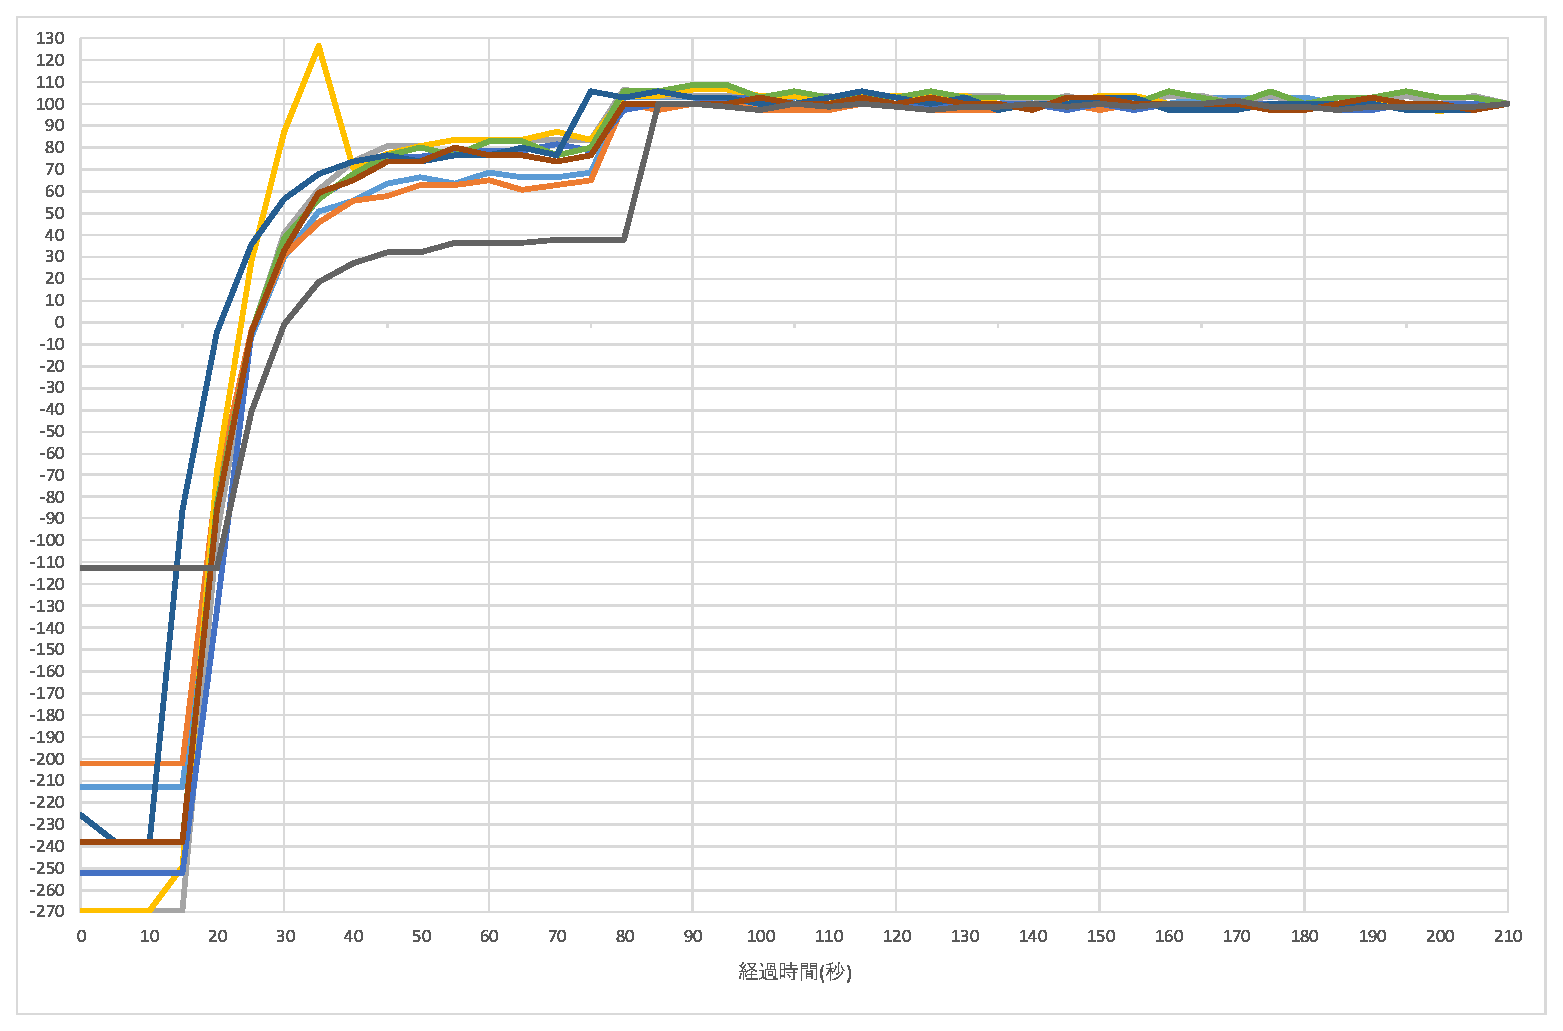
\includegraphics[width = 15cm]{./picture/co2_wait_graph.eps}
    \caption{二酸化炭素濃度センサの観測値の推移}
    \label{graph_co2_wait}
\end{figure}
%図\ref{graph_co2_wait}は横軸に通電開始からの経過時間,縦軸には二酸化炭素濃度0ppmを0として,各回の210秒後に観測された二酸化炭素濃度を100とした時の割合として二酸化炭素濃度を表した数値を示している.
図\ref{graph_co2_wait}は横軸に通電開始からの経過時間,縦軸には観測された二酸化炭素濃度を正規化したものを示している.
二酸化炭素濃度は複数回観測する中で環境を変えると210秒後における最終的な二酸化炭素濃度がそれぞれ異なっていたため,その値がすべて100になるように正規化を行っている.
縦軸で負の値が存在するのは,電圧が0ppmを表す基準電圧よりも低い電圧が観測することがあったため,そのまま二酸化炭素に比例するものとして算出しているためである.
この結果より,通電開始から90秒経過していれば,おおむね正規の値から前後10\%の範囲内の値が観測できることがうかがえる.
そこで,「センサヒートアップ待ち」状態は90秒で次の状態へ遷移するとした.
また,二酸化炭素濃度センサはアナログ電圧の計測時の誤差を少なくするために,10秒ごとに合計3回値の取得を行ったのちに,その平均値を用いて二酸化炭素濃度を推定することとした.
そして,それらをもとに,「時間待ち」状態から「センサヒートアップ待ち」状態へは70秒で推移することとした.

これらの時間の制定を受け,「夜間スリープ」状態を1日12時間制定した場合,1日で消費される推定電池容量の使用量を計算すると,約950mAhとなる.
アルカリ電池単3形を2本用いるとして,1本あたり100mAの連続放電が20時間\cite{denti}であることより,1本あたりの電池容量を2000mAhとすれば,乾電池2本で4日間以上使用可能であると考えられる.
これより,電池交換することなく12時間以上稼働するという設計を満たすことが期待できる.



% 第3章で述べた優先度の高い機能部分について実装を行った.本研究ではグループで開発を行った.サーバ側の精算システムを段原丞治が,Raspberry Piと各種センサを含むモビリティショッピング端末を筆者が実装した.Raspberry Pi はRaspberry Pi 3 Model Bを使用した.Raspberry Piの実装環境については,表\ref{rasp}に示す.


% \begin{table}[htb]
% \begin{center}
% \caption{Raspberry Pi環境}
% \begin{tabular}{|c||c|} \hline
% 使用機器 & Raspberry Pi3 Model B \\ \hline
% OS & raspbian9 \\ \hline
% CPU & 1.2GHz \\ \hline
% メモリ & 1GB \\ \hline
% \end{tabular}
% \label{rasp}
% \end{center}
% \end{table}


% Raspberry Piが制御した各種センサの実装環境について表\ref{jissou}に示す.


% \begin{table}[htb]
% \begin{center}
% \caption{実装環境}
% \begin{tabular}{|c|c|} \hline
% センサ & 個数 \\ \hline \hline
% ロジクール ウェブカメラ C615 & 1 \\
% HY-SRF05超音波距離センサモジュール & 1 \\
% ロードセル シングルポイント(ビーム型)3kg & 1 \\
% SODIAL(R) 100 5mm (LED) & 3 \\ \hline
% \end{tabular}
% \label{jissou}
% \end{center}
% \end{table}


% 上記のセンサをショッピングバスケットに取り付け,実装を行った.表\ref{jissou}に示した各種センサの選定については3.3節に述べたとおりである.ショッピングバスケットのサイズは33L,寸法はW510×D360×H240mmである.ショッピングバスケットを以下カゴと呼ぶ.また,対象の商品として,小規模店舗,中規模店舗にも取り扱いがありそうな菓子としてDARSとコアラのマーチを選定した.

% WebカメラはカゴのW510×D180×H150mmの位置に,カメラを底に向けて設置した.180×180mmのアクリル板をネジでロードセルに留め,Webカメラから100mm下に設置した.超音波センサの設置場所については,Webカメラと同じ高さの2種類の高さの両方の設置場所で実装した.LEDについては緑,青,赤の3色のLEDを抵抗と共にブレッドボードに設置した.カゴに実装したWebカメラ以外の各種センサについては図\ref{sensa}に示す.

% \begin{figure}[htbp]
% \centering
% \includegraphics[width = 15cm]{./picture/sensa_img.eps}
% \caption{各種センサ}
% \label{sensa}
% \end{figure}


% \subsection*{サーバとの通信}

% ユーザが商品を追加,削除した時のみに,Webカメラより画像を撮る.画像データの後に追加もしくは削除のフラグをセットにしてサーバへ送信する.送信のタイミングは3.4節で述べたメッセージにしたがう.

% \subsection*{各種センサの制御}

% それぞれのセンサを制御するためにpythonを開発言語として使用した.センサを稼働し続けるためにはループ処理を行う必要がある.しかしながら,ループ外でセンサが閾値を超えたか否かを確認する必要もあったため,センサの処理は別スレッドで動作させることとした.各センサは以下の動作をさせるよう実装した.

% \noindent
% {\bf ■超音波センサ}

% 商品,もしくは手を感知した際にフラグをたてる.システム起動の際,超音波センサからカゴの端までの距離を測り,その値を初期値とする.その初期値から値が減少していた場合フラグをたてる.ただし,初期値+30mmは誤差とする.

% \noindent
% {\bf ■Webカメラ}

% 超音波センサより,フラグがたった時に0.5秒に一度,合計6枚の画像を撮る.データ送信用配列にデータを追加する.

% \noindent
% {\bf ■ロードセル}

% 重量の増減を感知した際にフラグをたてる.増加したときに1のフラグを,減少した時に2のフラグをたてる.フラグをキューへ追加する.ただし,±3gの増減は誤差とする.

% \noindent
% {\bf ■LED}

% 超音波センサのフラグがたった時,画像撮影開始をユーザに知らせるために緑色のLEDを点灯させる.サーバへデータを送信後,バーコード情報を正しく読み取ることができたというフラグを受けとった際は青色のLEDを,読み取ることができなかったというフラグを受けとった際はユーザに再度商品の追加,削除を促すために赤色のLEDを点灯させる.

% \newpage


%Raspberry Pi側でしたこと